% !TEX root=/home/tavant/these/manuscript/src/manuscript.tex

\section{PIC simulation results: Boeuf model}


We start by presenting the results of the simulation case of Boeuf, since it is simpler to analyse.
Three different cases are presented.
The first is the usual case, without the effects of the radial direction.
It is expected to return the same results as obtained in \citet{boeuf2018}.
The two other cases model the radial effect of the radial direction.
Two values of the radial length are used\string: $L_R=4\,\centi\meter$ and $2\,\centi\meter$.

\subsection{Boeuf model: Temporal evolution} \label{subsec-temp_boeuf}

\Cref{fig-boeuf-temporal} present the temporal evolution of the mean plasma density and temperature.
We can see that when the radial direction is modeled, the density and the temperature is reduces as expected when increasing the losses.

\begin{figure}[hbtp]
  \centering
  \begin{tabular}{cc}
    \subfigure{Boeuf_ne_temporal}{a}{20,20} &
    \subfigure{Boeuf_Te_temporal}{b}{20,15} \\
  \end{tabular}
  \caption{({\bf a}) temporal evolution of the mean plasma density and  ({\bf b})  temporal evolution of the mean  electron temperature obtained with 3 different radial model for the simulation case of Boeuf. }
  \label{fig-boeuf-temporal}
\end{figure}

We can see on \cref{fig-boeuf-temporal}.{\bf b} that the radial temperature stays constant when the radial direction is not modeled.
this is due to the fact that the collisions are not modeled in the simulations, so that there is not momentum and energy transfer possible from the axial and azimuthal direction, and the radial direction.

However, we know from the radial-azimuthal simulations that there is a transfer, resulting in a plasma less anisotropic than observed here.
Consequently, the radial losses are far from the one expected in reality.


\subsection{Boeuf model: Axial profiles} \label{subsec-axial_boeuf}

Here: the axial profiles at steady state.

\begin{figure}[hbtp]
  \centering
  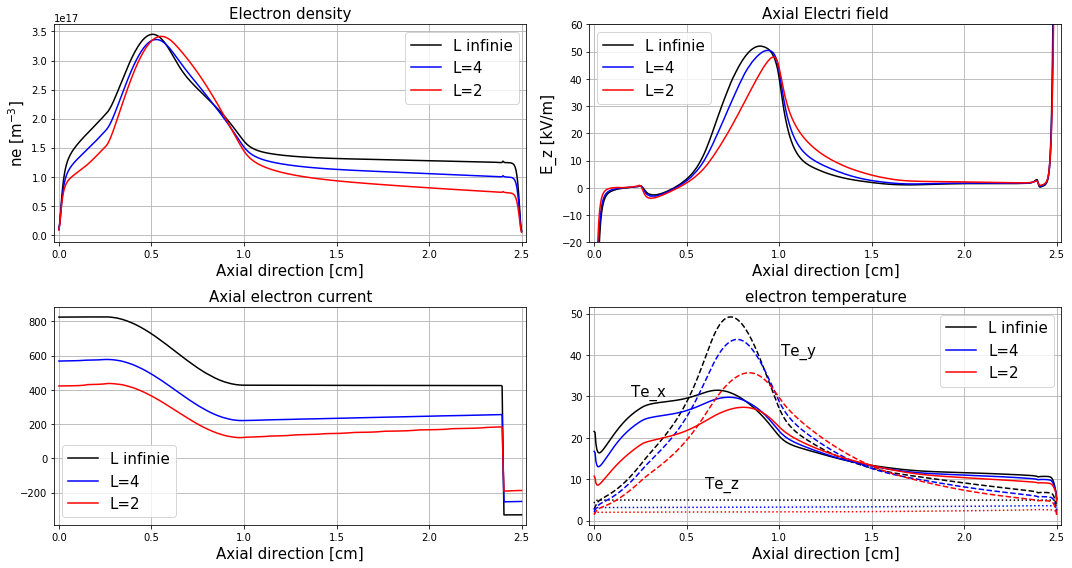
\includegraphics[width=\textwidth]{axial_profiles}
  \caption{Axial profiles of the final states for the plasma density, the axial electric field, the axial electron current and the electron mean temperature. }
  \label{fig-boeuf_axial}
\end{figure}

We see that the electron transport is highly affected.
This is expected to be due to the reduced electron temperature, which reduces the amplitude of the instability at saturation.
It is confirmed by \cref{fig-boeuf-instability}.

\begin{figure}[hbtp]
  \centering
  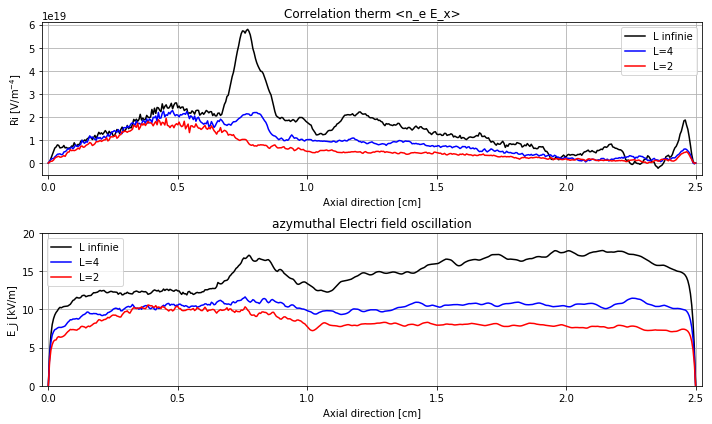
\includegraphics[width=\defaultwidth]{boeuf-axial-instability}
  \caption{Characteristics of the instability.}
  \label{fig-boeuf-instability}
\end{figure}

\inlinenote{Discussion of the role of the numerical noise, that could impact the instability as well.}

\subsection{Boeuf model: with MCC} \label{subsec-MCC_boeuf}
\inlinenote{We could add here the results of the Boeuf case with the MCC modeled.
See the value of $T_{e, R}$ and discuses on the heating indused by the waves. }